\documentclass[11pt]{article}
\usepackage{fullpage}
\usepackage{amssymb}
\usepackage{amsmath}
\usepackage{graphicx}
\usepackage{enumerate}
\usepackage{hyperref}
\usepackage[hyperref]{ntheorem}
\usepackage[noadjust]{cite}








\usepackage{tikz}
\usetikzlibrary{decorations.pathreplacing}
\usetikzlibrary{decorations.pathmorphing}
\usetikzlibrary{calc}
\usetikzlibrary{shapes.geometric}
\usetikzlibrary{shapes.misc}
\usetikzlibrary{positioning}
\usetikzlibrary{patterns}
\usetikzlibrary{fit}
\usetikzlibrary{arrows}
\usetikzlibrary{decorations.markings}


\tikzstyle{every picture}+=[remember picture]

\usepackage{subfig}
\captionsetup{lofdepth=2}

\newtheorem{theorem}{Theorem}
\newtheorem{lemma}{Lemma}
\providecommand*{\lemmaautorefname}{Lemma}
\newtheorem{corollary}{Corollary}
\providecommand*{\corollaryautorefname}{Corollary}
\newtheorem{definition}{Definition}
\newtheorem{prop}{Proposition}
\newcommand{\qed}{\hfill\ensuremath{\Box}\medskip\\\noindent}
\newenvironment{proof}{\noindent\emph{Proof. }}



\newcommand{\fingerprintq}{\ensuremath{\textsc{Fingerprint}}}
\newcommand{\lceq}{\ensuremath{\textsc{LCE}}}
\newcommand{\levelanc}{\ensuremath{\textsc{LA}}}
\renewcommand{\succ}{\ensuremath{\textsc{succ}}}
\newcommand{\pred}{\ensuremath{\textsc{pred}}}

\newcommand{\fp}{\ensuremath\phi}
\newcommand{\fpv}{\ensuremath{\phi_v}}
\newcommand{\fpe}{\ensuremath{\phi_e}}
\newcommand{\fpplus}{\ensuremath{\oplus}}
\newcommand{\fpdelsuffix}{\ensuremath{\ominus_s}}
\newcommand{\fpdelprefix}{\ensuremath{\ominus_p}}

\newcommand{\size}{\ensuremath{\mathit{size}}}
\newcommand{\depth}{\ensuremath{\mathit{depth}}}
\newcommand{\leaf}{\ensuremath{\mathit{leaf}}}
\newcommand{\heavy}{\ensuremath{heavy}}
\newcommand{\heavypath}{\ensuremath{H}}
\newcommand{\rootnode}{\ensuremath{\mathit{root}}}
\newcommand{\lchild}{\ensuremath{\mathit{left}}}
\newcommand{\rchild}{\ensuremath{\mathit{right}}}
\newcommand{\leftnodes}{\ensuremath{V}} \newcommand{\leftsize}{\ensuremath{L}} \newcommand{\leftstring}{\ensuremath{P}} \newcommand{\str}{\ensuremath{S} }
\newcommand{\slp}{\ensuremath{G} }
\newcommand{\lslp}{\ensuremath{G_L} }

\newcommand{\lce}{\ensuremath\ell}
\newcommand{\rs}{root-substring}

\title{Fingerprints in Compressed Strings\footnote{An extended abstract of this paper appeared at the 13th Algorithms and Data Structures Symposium.}}
\author{Philip Bille \\ \texttt{phbi@dtu.dk} \and Patrick Hagge Cording \\ \texttt{phaco@dtu.dk} \and Inge Li G{\o}rtz\thanks{Supported by a grant from the Danish Council for Independent Research  Natural Sciences.} \\ \texttt{inge@dtu.dk} \and Benjamin Sach \\ \texttt{sach@dcs.warwick.ac.uk} \and Hjalte Wedel Vildh{\o}j \\ \texttt{hwvi@dtu.dk} \and S{\o}ren Vind\thanks{Supported by a grant from the Danish National Advanced Technology Foundation.} \\ \texttt{sovi@dtu.dk}}


\begin{document}
	
\maketitle

\begin{abstract}
\noindent The Karp-Rabin fingerprint of a string is a type of hash value that due to its strong properties has been used in many string algorithms. In this paper we show how to construct a data structure for a string  of size  compressed by a context-free grammar of size  that answers fingerprint queries. That is, given indices  and , the answer to a query is the fingerprint of the substring . We present the first  space data structures that answer fingerprint queries without decompressing any characters. For Straight Line Programs (SLP) we get  query time, and for Linear SLPs (an SLP derivative that captures LZ78 compression and its variations) we get  query time. Hence, our data structures has the same time and space complexity as for random access in SLPs. We utilize the fingerprint data structures to solve the longest common extension problem in query time  and  for SLPs and Linear SLPs, respectively. Here,  denotes the length of the LCE.
\end{abstract}


\section{Introduction}
Given a string \str of size  and a Karp-Rabin fingerprint function , the answer to a  query is the fingerprint  of the substring . We consider the problem of constructing a data structure that efficiently answers fingerprint queries when the string is compressed by a context-free grammar of size .

The fingerprint of a string is an alternative representation that is much shorter than the string itself. By choosing the fingerprint function randomly at runtime it exhibits strong guarantees for the probability of two different strings having different fingerprints. Fingerprints were introduced by Karp and Rabin~\cite{karp1987efficient} and used to design a randomized string matching algorithm. Since then, they have been used as a central tool to design algorithms for a wide range of problems (see e.g.,~\cite{amir1992efficient, andoni2006efficient, cole2003faster, cormode2005substring, cormode2007string, farach1998string, gasieniec1996randomized, kalai2002efficient, porat2009exact}). 

A fingerprint requires constant space and it has the useful property that given the fingerprints  and , the fingerprint  can be computed in constant time. By storing the fingerprints  for  a query can be answered in  time. However, this data structure uses  space which can be exponential in . Another approach is to use the data structure of G\c{a}sieniec~et~al.~\cite{gasieniec2005real} which supports linear time decompression of a prefix or suffix of the string generated by a node. To answer a query we find the deepest node that generates a string containing  and  and decompress the appropriate suffix of its left child and prefix of its right child. Consequently, the space usage is  and the query time is , where  is the height of the grammar. The  time to find the correct node can be improved to  using the data structure by Bille et al.~\cite{bille2011random} giving  time for a  query. Note that the query time depends on the length of the decompressed string which can be large.

We present the first data structures that answers fingerprint queries on grammar compressed strings without decompressing any characters, and improve all of the above time-space trade-offs. Assume without loss of generality that the compressed string is given as a Straight Line Program (SLP). An SLP is a grammar in Chomsky normal form, i.e., each nonterminal has exactly two children. A Linear SLP is an SLP where the root is allowed to have more than two children, and for all other internal nodes, the right child must be a leaf. Linear SLPs capture the LZ78 compression scheme~\cite{lz78} and its variations. Our data structures give the following theorem.

\begin{theorem}\label{thm:fp}
	Let  be a string of length  compressed into an SLP  of size~. We can construct data structures that support  queries in:
	\begin{enumerate}
		\item[(i)]  space and query time 
		\item[(ii)]  space and query time  if  is a Linear SLP
	\end{enumerate}
\end{theorem}

\noindent Hence, we show a data structure for fingerprint queries that has the same time and space complexity as for random access in SLPs. 

Our fingerprint data structures are based on the idea that a random access query for  produces a path from the root to a leaf labelled . The concatenation of the substrings produced by the left children of the nodes on this path produce the prefix . We store the fingerprints of the strings produced by each node and concatenate these to get the fingerprint of the prefix instead. For \autoref{thm:fp}(i), we combine this with the fast random access data structure by Bille et al.~\cite{bille2011random}. For Linear SLPs we use the fact that the production rules form a tree to do large jumps in the SLP in constant time using a level ancestor data structure. Then a random access query is dominated by finding the node that produces  among the children of the root, which can be modelled as the predecessor problem.

Furthermore, we show how to obtain faster query time in Linear SLPs using finger searching techniques. Specifically, a finger for position  in a Linear SLP is a pointer to the child of the root that produces .



\begin{theorem}\label{thm:ffp}
Let  be a string of length  compressed into an SLP  of size~. We can construct an  space data structure such that given a finger  for position  or , we can answer a  query in time  where .
\end{theorem}

\noindent Along the way we give a new and simple reduction for solving the finger predecessor problem on integers using any predecessor data structure as a black~box.





In compliance with all related work on grammar compressed strings, we assume that the model of computation is the RAM model with a word size of  bits.




\subsection{Longest common extension in compressed strings}
As an application we show how to efficiently solve the longest common extension problem (LCE).
Given two indices  in a string , the answer to the  query is the length  of the maximum substring such that . The compressed LCE problem is to preprocess a compressed string to support LCE queries. On uncompressed strings this is solvable in  preprocessing time,  space, and  query time with a nearest common ancestor data structure on the suffix tree for  \cite{HT1984}. Other trade-offs are obtained by doing an exponential search over the fingerprints of strings starting in  and  \cite{bille12lce}. Using the exponential search in combination with the previously mentioned methods for obtaining fingerprints without decompressing the entire string we get  or  time using  space for an LCE query. Using our new (finger) fingerprint data structures and the exponential search we obtain \autoref{thm:lce}.

\begin{theorem}\label{thm:lce}
Let  be an SLP of size  that produces a string  of length . The SLP  can be preprocessed in  time into a Monte Carlo data structure of size  that supports LCE queries on  in
\begin{enumerate}
\item[(i)]  time
\item[(ii)]  time if  is a Linear SLP.
\end{enumerate}
Here  denotes the LCE value and queries are answered correctly with high probability. Moreover, a Las Vegas version of both data structures that always answers queries correctly can be obtained with
 preprocessing time with high probability.
\end{theorem}



	


\noindent We furthermore show how to reduce the Las Vegas preprocessing time to  when all the internal nodes in the Linear SLP are children of the root (which is the case in LZ78).

The following corollary follows immediately because an LZ77 compression~\cite{lz77} consisting of  phrases can be transformed to an SLP with  production rules~\cite{charikar2005smallest,rytter2003application}.

\begin{corollary}
	We can solve the  problem in  space and query time  for LZ77 compression.
\end{corollary}

\noindent Finally, the LZ78 compression can be modelled by a Linear SLP  with constant overhead. Consider an LZ78 compression with  phrases, denoted . A terminal phrase corresponds to a leaf in , and each phrase , , corresponds to a node  with  corresponding to the left child of  and the right child of  being the leaf corresponding to . Therefore, we get the following corollary.

\begin{corollary}
	We can solve the  problem in  space and query time  for LZ78 compression.
\end{corollary}

\section{Preliminaries}
Let  be a string of length . Denote by  the character in  at index  and let  be the substring of  of length  from index  to , both indices included.

A Straight Line Program (SLP)  is a context-free grammar in Chomsky normal form that we represent as a node-labeled and ordered directed acyclic graph. Each leaf in  is labelled with a character, and corresponds to a terminal grammar production rule. Each internal node in  is labeled with a nonterminal rule from the grammar. The unique string  of length  is \emph{produced} by a depth-first left-to-right traversal of  and consist of the characters on the leafs in the order they are visited. We let  denote the root of , and  and  denote the left and right child of an internal node , respectively.

A Linear SLP  is an SLP where we allow  to have more than two children. All other internal nodes  have a leaf as . Although similar, this is not the same definition as given for the Relaxed SLP by Claude and Navarro~\cite{claude2011self}. The Linear SLP is more restricted since the right child of any node (except the root) must be a leaf. Any Linear SLP can be transformed into an SLP of at most double size by adding a new rule for each child of the root.

We extend the classic \emph{heavy path decomposition} of Harel and Tarjan \cite{HT1984} to SLPs as in \cite{bille2011random}. For each node , we select one edge from  to a child with maximum size and call it the \emph{heavy edge}. The remaining edges are \emph{light edges}. Observe that  if  is a parent of  and the edge connecting them is light. Thus, the number of light edges on any path from the root to a leaf is at most . 
A \emph{heavy path} is a path where all edges are heavy. The heavy path of a node , denoted , is the unique path of heavy edges starting at . Since all nodes only have a single outgoing heavy edge, the heavy path  and its leaf , is well-defined for each node .




A \emph{predecessor data structure} supports predecessor and successor queries on a set  of  integers from a universe  of size . The answer to a \emph{predecessor query}  is the largest integer  such that , while the answer to a \emph{successor query}  is the smallest integer  such that . There exist predecessor data structures achieving a query time of  using space  \cite{van1976design, mehlhorn1990bounded, willard1983log}.

Given a rooted tree  with  vertices, we let  denote the length of the path from the root of  to a node . A \emph{level ancestor data structure} on  supports \emph{level ancestor queries} , asking for the ancestor  of  such that . There is a level ancestor data structure answering queries in  time using  space \cite{dietz1991finding} (see also \cite{berkman1994finding, alstrup2000improved, bender2004level}).

\subsection{Fingerprinting}
The Karp-Rabin fingerprint \cite{karp1987efficient} of a string  is defined as , where  is a randomly chosen positive integer, and  is a prime. Karp-Rabin fingerprints guarantee that given two strings  and , if  then . Furthermore, if , then with high probability . Fingerprints can be composed and subtracted as follows.

\begin{lemma}\label{lem:fp}
Let  be a string decomposable into a prefix  and suffix . Let  be the maximum length of ,  be a random integer and  be a prime. Given any two of the Karp-Rabin fingerprints ,  and , it is possible to calculate the remaining fingerprint in constant time as follows:

\end{lemma}

\noindent In order to calculate the fingerprints of \autoref{lem:fp} in constant time, each fingerprint for a string  must also store the associated exponent , and we will assume this is always the case. Observe that a fingerprint for any substring  of a string can be calculated by subtracting the two fingerprints for the prefixes  and . Hence, we will only show how to find fingerprints for prefixes in this paper.

\section{Basic fingerprint queries in SLPs}
We now describe a simple data structure for answering  queries for a string  compressed into a SLP  in time , where  is the height of the parse tree for . This method does not unpack the string to obtain the fingerprint, instead the fingerprint is generated by traversing . 



The data structure stores  and the fingerprint  of the string produced by each node . To compose the fingerprint  we start from the root of \slp and do the following. Let  denote the currently visited node, and let  be a variable denoting the size the concatenation of strings produced by left children of visited nodes. We follow an edge to the right child of  if , and follow a left edge otherwise. If following a right edge, update  such that the fingerprint of the full string generated by the left child of  is added to , and set . When following a left edge,  and  remains unchanged. When a leaf is reached, let  to include the fingerprint of the terminal character. Aside from the concatenation of fingerprints for substrings, this procedure resembles a random access query for the character in position  of .









The procedure correctly composes  because the order in which the fingerprints for the substrings are added to  is identical to the order in which the substrings are decompressed when decompressing . 

Since the fingerprint composition takes constant time per addition, the time spent generating a fingerprint using this method is bounded by the height of the parse tree for , denoted . Only constant additional space is spent for each node in , so the space usage is .

\section{Faster fingerprints in SLPs}
Using the data structure of Bille et al.~\cite{bille2011random} to perform random access queries allows for a faster way to answer  queries.



\begin{lemma}[\cite{bille2011random}]\label{lem:slp:random}
Let  be a string of length  compressed into a SLP  of size . Given a node , we can support random access in  in  time, at the same time reporting the sequence of heavy paths and their entry- and exit points in the corresponding depth-first traversal of .
\end{lemma}

\noindent The main idea is to compose the final fingerprint from substring fingerprints by performing a constant number of fingerprint additions per heavy path visited.


\begin{figure}[tb]
	
	\begin{center}
	\begin{tikzpicture}[x=1,y=1,-,>=stealth',auto, thick,
every label/.style={inner sep=3pt},
	tnode/.style={draw=black, fill=white, circle, inner sep=0pt, minimum size=4pt},
  	terminal/.style={circle,fill=white, inner sep=0.2pt},
  	box/.style={minimum height=11,minimum width=40, inner sep=1},
  	subtree/.style={thin,draw}]

\def\spacing{18}

\draw [] (60,-6) rectangle (120,6);
\foreach \x in {100}{
	\draw [] (\x,-6) -- (\x,6);
}

\draw [] (20,-6+1*\spacing) rectangle (120,6+1*\spacing);
\foreach \x in {60,100}{
	\draw [] (\x,-6+1*\spacing) -- (\x,6+1*\spacing);
}

\draw [] (20,-6+3*\spacing) rectangle (220,6+3*\spacing);
\foreach \x in {100,120,140}{
	\draw [] (\x,-6+2*\spacing) -- (\x,6+2*\spacing);
}

\draw [] (60,-6+2*\spacing) rectangle (180,6+2*\spacing);
\foreach \x in {60,100,120,140,180}{
	\draw [] (\x,-6+3*\spacing) -- (\x,6+3*\spacing);
}

\node[minimum width=40] at (0,2*\spacing) {};
\node[box] at (80,2*\spacing) {};
\node[box,minimum width=20] at (230,2*\spacing) {};
\node[box] at (160,2*\spacing) {};

\node[minimum width=40] at (0,3*\spacing) {};
\node[box] at (40,3*\spacing) {};
\node[box] at (80,3*\spacing) {};
\node[box,minimum width=20] at (230,3*\spacing) {};
\node[box] at (160,3*\spacing) {};
\node[box] at (200,3*\spacing) {};

\node[minimum width=40] at (0,\spacing) {};
\node[box] at (40,\spacing) {};
\node[box] at (80,\spacing) {};


\node[minimum width=40] at (0,0) {};
\node[box] at (80,0) {};




\def\nodeyoffset{10}

\node[tnode, label=left:] (a) at (40, 200+\nodeyoffset) {};
\node[tnode, label=left:] (b) at (80, 150+\nodeyoffset) {};
\node[tnode, label=left:] (c) at (110, 80+\nodeyoffset) {};
\node[tnode, label=right:] (d) at (200, 170+\nodeyoffset) {};
\node[tnode, label=right:] (e) at (160, 140+\nodeyoffset) {};

\def\subtreeheight{35}

\path[subtree] (a) -- () -- () -- (a);
\path[subtree] (b) -- () -- () -- (b);
\path[subtree] (d) -- () -- () -- (d);
\path[subtree] (e) -- () -- () -- (e);




\node[tnode, label=left:] (f) at () {};
\node[tnode] (g) at () {};
\node[tnode, label=left:] (h) at () {};
\node[tnode] (i) at () {};
\node[tnode] (j) at () {};
\node[tnode] (k) at () {};

\path[draw] (f) -- (g) -- (h) -- (i) -- (j) -- (k);
\path[draw, dashed] (a) -- (f);
\path[draw, dashed] (b) -- (h);
\path[draw, dashed] (c) -- (j);
\path[draw, dashed] (d) -- (g);
\path[draw, dashed] (e) -- (i);

\draw[decorate,decoration={brace,raise=0pt,amplitude=3pt}] (120,84) -- (20,84) node[midway,label={[label distance=-4]below:}] {};

\node[] (leaf) at () {};
\path[->,>=stealth',auto,thin,shorten >=5] (leaf) edge [] (k);
\path[->,>=stealth',auto,thin,shorten >=5] (leaf) edge [] (130,6+3*\spacing);

\node[] (d1) at () {};
\node[] (d2) at () {};
\node[] (d3) at () {};

\path[draw,decorate,decoration={snake,amplitude=0.3mm,segment length=4mm,pre length=0mm, post length=0mm}] (d1) -- (f);
\path[draw,decorate,decoration={snake,amplitude=0.3mm,segment length=4mm,pre length=0mm, post length=0mm}] (d2) -- (f);
\path[draw,decorate,decoration={snake,amplitude=0.3mm,segment length=4mm,pre length=0mm, post length=0mm}] (d3) -- (g);


\end{tikzpicture}	
	\end{center}
	\caption{Figure showing how  and its prefix  is composed of substrings generated by the left children  and right children  of the heavy path . Also illustrates how this relates to  and  for a node .\label{fig:slp:strings}}
\end{figure}

In order to describe the data structure, we will use the following notation. Let  be the left children of the nodes in  where the heavy path was extended to the right child, ordered by increasing depth. The order of nodes in  is equal to the sequence in which they occur when decompressing , so the concatenation of the strings produced by nodes in  yields the prefix , where . Observe that  is a suffix of  if . See \autoref{fig:slp:strings} for the relationship between ,  and the defined strings.
 
Let each node  store its unique outgoing heavy path , the length , , and the fingerprints  and . By forming heavy path trees of total size  as in \cite{bille2011random}, we can store  as a pointer to a node in a heavy path tree (instead of each node storing the full sequence).

The fingerprint  is composed from the sequence of heavy paths visited when performing a single random access query for  using \autoref{lem:slp:random}. Instead of adding all left-children of the path towards  to  individually, we show how to add all left-children hanging from each visited heavy path in constant time per heavy path. Thus, the time taken to compose  is . 

More precisely, for the pair of entry- and exit-nodes  on each heavy path  traversed from the root to , we set  (which is allowed because  is a suffix of ). If we leave  by following a right-pointer, we additionally set . If  is a leaf, set  to include the fingerprint of the terminal character. 

Remember that  is exactly the string generated from  along , produced by the left children of nodes on  where the heavy path was extended to the right child. Thus, this method corresponds exactly to adding the fingerprint for the substrings generated by all left children of nodes on  between the entry- and exit-nodes in depth-first order, and the argument for correctness from the slower fingerprint generation also applies here.

Since the fingerprint composition takes constant time per addition, the time spent generating a fingerprint using this method is bounded by the number of heavy paths traversed, which is . Only constant additional space is spent for each node in , so the space usage is . This concludes the proof of \autoref{thm:fp}(i).

\section{Faster fingerprints in Linear SLPs}
In this section we show how to quickly answer  queries on a Linear SLP . In the following we denote the sequence of  children of  from left to right by . Also, let  for . That is,  is the length of the prefix of  produced by  including  (and  is the empty prefix).

We also define the dictionary tree  over  as follows. Each node  corresponds to a single vertex . There is an edge  labeled  if  and . If  is a leaf, there is an edge  labeled . That is, a left child edge of  is converted to a parent edge of  labeled like the right child leaf of . Note that for any node  except the root, producing  is equivalent to following edges and reporting edge labels on the path from  to . Thus, the prefix of length  of  may be produced by reporting the edge labels on the path from  until reaching the ancestor of  at depth .


\begin{figure}[tb]
\begin{center}
\subfloat[Linear SLP.]{
\pgfdeclarelayer{background layer}
\pgfdeclarelayer{foreground layer}
\pgfsetlayers{background layer,main,foreground layer}
\begin{tikzpicture}[->,>=stealth',auto, thick,
every label/.style={rectangle, rounded corners, font=\scriptsize, line width=5pt, inner sep=1pt, fill=white, fill opacity=0.9, text opacity=1.0},
	main node/.style={draw=black, fill=white, circle, inner sep=0pt, minimum size=4pt},
  	terminal/.style={rectangle,text height=7pt, fill=white, inner sep=0.2pt}]



\node[main node] (root) [] {};
  \node[main node, label=left:] (1) [below left=1.6cm and 2.5cm of root] {};
  \node[main node, label=left:] (2) [below left=1.6cm and 1.5cm of root] {};
  \node[main node, label=left:] (3) [below left=1.6cm and 0.5cm of root] {};
  \node[main node, label=left:] (4) [below right=1.6cm and 0.5cm of root] {};
  \node[main node, label=left:] (5) [below right=1.6cm and 1.5cm of root] {};
  \node[main node, label=left:] (6) [below right=1.6cm and 2.5cm of root] {};

  \node[terminal] (a1) [below=1cm of 1] {};
  \node[terminal] (a2) [below=1cm of 3] {};
  \node[terminal] (a3) [below=1cm of 5] {};
\node[terminal] (b1) [below=1cm of 2] {};
  \node[terminal] (b2) [below=1cm of 4] {};
  \node[terminal] (b3) [below=1cm of 6] {};


  \begin{pgfonlayer}{background layer}
  \path[] (root) edge [] (1);
  \path[] (root) edge [] (2);
  \path[] (root) edge [] (3);
  \path[] (root) edge [] (4);
  \path[] (root) edge [] (5);
  \path[] (root) edge [] (6);

  \path[] (1) edge [] (a1);
  \path[] (3) edge [] (a2);
  \path[] (5) edge [] (a3);
  \path[] (2) edge [] (b1);
  \path[] (4) edge [] (b2);
  \path[] (6) edge [] (b3);

  \path[] (3) edge [bend left] (2);
  \path[] (4) edge [bend left] (1);
  \path[] (5) edge [bend left=20] (3);
  \path[] (6) edge [bend left=50] (3);

\end{pgfonlayer}{background layer}
\end{tikzpicture}
}\quad\quad\quad\quad\subfloat[Dictionary tree.]{
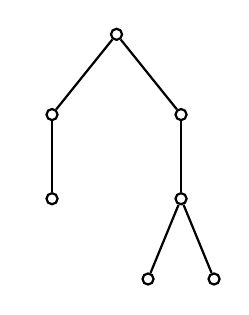
\begin{tikzpicture}[-,>=stealth',auto, thick,
every label/.style={rectangle, font=\scriptsize, inner sep=3pt},
	main node/.style={draw=black, fill=white, circle, inner sep=0pt, minimum size=4pt},
  	terminal/.style={circle,fill=white, inner sep=0.2pt}]

  \node[main node] (root) [] {};
  \node[main node, label=left:] (1) [below left=0.9cm and 0.7cm of root] {};
  \node[main node, label=left:] (2) [below right=0.9cm and 0.7cm of root] {};
  \node[main node, label=left:] (3) [below=0.9cm of 2] {};
  \node[main node, label=left:] (4) [below=0.9cm of 1] {};
  \node[main node, label=left:] (5) [below left=0.9cm and 0.3cm of 3] {};
  \node[main node, label=left:] (6) [below right=0.9cm and 0.3cm of 3] {};

  \path[] (root) edge [] node [left] {} (1);
  \path[] (root) edge [] node [right] {} (2);
  \path[] (1) edge [] node [left] {} (4);
  \path[] (3) edge [] node [left] {} (5);
  \path[] (2) edge [] node [right] {} (3);
  \path[] (3) edge [] node [right] {} (6);
\end{tikzpicture}	
}

\caption{A Linear SLP compressing the string \texttt{abbaabbaabab} and the dictionary tree obtained from the Linear SLP.}\label{fig:linslpex1}

\end{center}
\end{figure}

The data structure stores a predecessor data structure over the prefix lengths  and the associated node  and fingerprint  for . We also have a doubly linked list of all 's with bidirectional pointers to the predecessor data structure and .  We store the dictionary tree  over , augment it with a level ancestor data structure, and add bidirectional pointers between  and . Finally, for each node , we store the fingerprint of the string it produces, . 

A query  is answered as follows. Let  be the predecessor of  among . Compose the answer to  from the two fingerprints . The first fingerprint  is stored in the data structure and the second fingerprint  can be found as follows. Observe that  is fully generated by  and hence a prefix of  of length . We can get  in constant time from  using the doubly linked list. We use a level ancestor query  to determine the ancestor of  at depth , corresponding to a prefix of  of the correct length. From  we can find .

It takes constant time to find  using a single level ancestor query and following pointers. Thus, the time to answer a query is bounded by the time spent determining , which requires a predecessor query among  elements (i.e. the number of children of ) from a universe of size . The data structure uses  space, as there is a bijection between nodes in  and vertices in , and we only spend constant additional space per node in  and vertex in . This concludes the proof of \autoref{thm:fp}(ii).


\section{Finger fingerprints in Linear SLPs}
The  running time of a  query is dominated by having to find the predecessor  of  among . Given  the rest of the query takes constant time. In the following, we show how to improve the running time of a  query to  given a finger for position .  Recall that a finger  for  a position  is a pointer to the node  producing .
To achieve this, we present a simple linear space finger predecessor data structure that is interchangeable with any other predecessor data structure.

\subsection{Finger Predecessor}
Let  be a set of  integers from a universe  of size . Given a finger  and a query point , the \emph{finger predecessor problem} is to answer finger predecessor or successor queries in time depending on the universe distance  from the finger to the query point. Belazzougui et al.~\cite{fingerpred} present a succinct solution for solving the finger predecessor problem relying on a modification of z-fast tries. Here, we use a simple reduction for solving the finger predecessor problem using any predecessor data structure as a black box. 

\begin{lemma}\label{lem:fingerpred}
	Let  be a set of  integers from a universe  of size . 
	Given a predecessor data structure with query time  using  space,
	we can solve the finger predecessor problem in time  using space .
\end{lemma}
\begin{proof}
Construct a complete balanced binary search tree  over the universe . The leaves of  represent the integers in , and we say that a vertex \emph{span} the range of  represented by the leaves in its subtree. Mark the leaves of  representing the integers in . We remove all vertices in  where the subtree contains no marked vertices. Observe that a vertex at height  span a universe range of size . We augment  with a level ancestor data structure answering queries in constant time. Finally, left- and right-neighbour pointers are added for all nodes in .

Each internal node  at height  store an instance of the given predecessor data structure for the set of marked leaves in the subtree of . The size of the universe for the predecessor data structure equals the span of the vertex and is \footnote{The integers stored by the data structure may be shifted by some constant  for a vertex at height , but we can shift all queries by the same constant and thus the size of the universe is .}.

Given a finger  and a query point , we will now describe how to find both  and  when . The case  is symmetric. 
Observe that  corresponds to a leaf in , denoted . We answer a query by determining the ancestor  of  at height  and its left neighbour  (if it exists). We query for  in the predecessor data structures of both  and , finding at least one leaf in  (since  spans  and ). We return the leaf representing the smallest result as  and its left neighbour in  as .

Observe that the predecessor data structures in  and  each span a universe of size . All other operations performed take constant time. Thus, for a predecessor data structure with query time , we can answer finger predecessor queries in time .

The height of  is , and there are  vertices in  (since vertices spanning no elements from  are removed). Each element from  is stored in  predecessor data structures. Hence, given a predecessor data structure with space usage , the total space usage of the data structure is . 

We reduce the size of the data structure by reducing the number of elements it stores to . This is done by partitioning  into  sets of consecutive elements  of size . We choose the largest integer in each  set as the representative  for that set, and store that in the data structure described above. We store the integers in set  in an atomic heap \cite{fredmanwillardfusion, Hagerup1998} capable of answering predecessor queries in  time and linear space for a set of size . Each element in  keep a pointer to the set  it belongs to, and each set left- and right-neighbour pointers.

Given a finger  and a query point , we describe how to determine  and  when . The case  is symmetric. We first determine the closest representatives  and  on the left and right of , respectively. Assuming , we proceed as before using  as the finger into  and query point . This gives  and  among the representatives. If  is undefined or , we select  and .
To produce the final answers, we perform at most 4 queries in the atomic heaps that  and  are representatives for. 

All queries in the atomic heaps take constant time, and we can find  and  in constant time by following pointers. If we query a predecessor data structure, we know that the range it spans is  since . Thus, given a predecessor data structure with query time , we can solve the finger predecessor problem in time .

The total space spent on the atomic heaps is  since they partition . The number of representatives is . Thus, given a predecessor data structure with space usage , we can solve the finger predecessor problem in space .\qed
\end{proof}

\noindent Using the van Emde Boas predecessor data structure \cite{van1976design, mehlhorn1990bounded, willard1983log} with  query time using  space, we obtain the following corollary.

\begin{corollary}\label{cor:fingerpred}
	Let  be a set of  integers from a universe  of size . 
	Given a finger  and a query point , we can solve the finger predecessor problem in time  and space .\end{corollary}

\subsection{Finger Fingerprints}
We can now prove Theorem~\ref{thm:ffp}. Assume wlog that we have a finger for , i.e., we  are given a finger  to the node  generating . From this we can in constant time get a pointer to  in the doubly linked list and from this a pointer to  in the predecessor data structure. If  then  is the predecessor of . Otherwise,  using Corollary~\ref{cor:fingerpred} we can in time  find the predecessor of . Since  and the rest of the query takes constant time, the total time for the query is .




\section{Longest Common Extensions in Compressed Strings}
Given an SLP , the longest common extension (LCE) problem is to build a data structure for  that supports longest common extension queries . In this section we show how to use our fingerprint data structures as a tool for doing LCE queries and hereby obtain \autoref{thm:lce}.



\subsection{Computing Longest Common Extensions with Fingerprints}


We start by showing the following general lemma that establishes the connection between LCE and fingerprint queries.

\begin{lemma}\label{lem:lce-comparisons}
For any string  and any partition  of  into  non-empty substrings called phrases,  can be found by comparing  pairs of substrings of  for equality. Furthermore, all substring comparisons  are of one of the following two types:
\begin{description}
\item[Type 1] Both  and  are fully contained in (possibly different) phrase substrings.
\item[Type 2]  for some  and for  or  it holds that
\begin{enumerate}
\item[(a)] The start position is also the start position of a phrase substring, or
\item[(b)] The end position is also the end position of a phrase substring.
\end{enumerate}
\end{description}
\end{lemma}
\begin{proof}
Let a position of  be a \emph{start} (\emph{end}) position if a phrase starts (ends) at that position. Moreover, let a comparison of two substrings be of \emph{type 1} (\emph{type 2}) if it satisfies the first (second) property in the lemma. We now describe how to find  by using  type 1 or 2 comparisons.

If  or  is not a start position, we first check if  (type 1), where  is the minimum integer such that  or  is an end position. If the comparison fails, we have restricted the search for  to two phrase substrings, and we can find the exact value using  type 1 comparisons.

Otherwise,  and either  or  is a start position. This leaves us with the task of describing how to answer , assuming that either  or  is a start position.

We first use  type 2 comparisons to determine the biggest integer  such that . It follows that . Now let  denote the length of the longest common prefix of the substrings  and , both of length . Clearly, . By comparing the first half  of  to the first half  of , we can determine if  or . By recursing we obtain the exact value of  after  comparisons.

However, comparing  and  directly is not guaranteed to be of type 1 or 2. To fix this, we compare them indirectly using a type 1 and type 2 comparison as follows. Let  be the minimum integer such that  or  is a start position. If there is no such  then we can compare  and  directly as a type 1 comparison. Otherwise, it holds that  if and only if  (type 1) and  (type 2).
\qed
\end{proof}


\noindent \autoref{thm:lce} follows by using fingerprints to perform the substring comparisons. In particular, we obtain a Monte Carlo data structure that can answer a LCE query in  time for SLPs and in  time for Linear SLPs. In the latter case, we can use \autoref{thm:ffp} to reduce the query time to  by observing that for all but the first fingerprint query, we have a finger into the data structure. 






\subsection{Verifying the Fingerprint Function}
Since the data structure is Monte Carlo, there may be collisions among the fingerprints used to determine the LCE, and consequently the answer to a query may be incorrect. We now describe how to obtain a Las Vegas data structure that always answers LCE queries correctly. We do so by showing how to efficiently verify that the fingerprint function  is , i.e., collision-free on all substrings compared in the computation of . We give two verification algorithms. One that works for LCE queries in SLPs, and a faster one that works for Linear SLPs where all internal nodes are children of the root (e.g. LZ78).






\subsubsection{SLPs}
If we let the phrases of  be its individual characters, we can assume that all fingerprint comparisons are of type 2 (see \autoref{lem:lce-comparisons}). We thus only have to check that  is collision-free among all substrings of length . We verify this in  rounds. In round  we maintain the fingerprint of a sliding window of length  over . For each substring  we insert  into a dictionary. If the dictionary already contains a fingerprint , we verify that  in constant time by checking if  and . This works because we have already verified that the fingerprinting function is collision-free for substrings of length . Note that we can assume that for any fingerprint  the fingerprints of the first and last half of  are available in constant time, since we can store and maintain these at no extra cost. In the first round , we check that  by comparing the two characters explicitly. If  we have found a collision and we abort and report that  is not good. If all rounds are successfully verified, we report that  is good.

For the analysis, observe that computing all fingerprints of length  in the sliding window can be implemented by a single traversal of the SLP parse tree in  time. Thus, the algorithm correctly decides whether  is good in  time and  space. We can easily reduce the space to  by carrying out each round in  iterations, where no more than  fingerprints are stored in the dictionary in each iteration. So, alternatively,  can be verified in  time and  space.

\subsubsection{Linear SLPs} In Linear SLPs where all internal nodes are children of the root, we can reduce the verification time to , while still using  space. To do so, we use \autoref{lem:lce-comparisons} with the partition of  being the root substrings. We verify that  is collision-free for type 1 and type 2 comparisons separately.


\paragraph{Type 1 Comparisons.}
We carry out the verification in rounds. In round  we check that no collisions occur among the -length substrings of the root substrings as follows: We traverse the SLP maintaining the fingerprint of all -length substrings. For each substring  of length , we insert  into a dictionary. If the dictionary already contains a fingerprint  we verify that  in constant time by checking if  and  (type 1).

Every substring of a root substring ends in a leaf in the SLP and is thus a suffix of a root substring. Consequently, they can be generated by a bottom up traversal of the SLP. The substrings of length 1 are exactly the leaves. Having generated the substrings of length , the substrings of length  are obtained by following the parents left child to another root node and prepending its right child. In each round the  length substrings correspond to a subset of the root nodes, so the dictionary never holds more than  fingerprints. Furthermore, since each substring is a suffix of a root substring, and the root substrings have at most  suffixes in total, the algorithm will terminate in  time.


\paragraph{Type 2 Comparisons.}
We adopt an approach similar to that for SLPs and verify  in  rounds. In round  we store the fingerprints of the substrings of length  that start or end at a phrase boundary in a dictionary. We then slide a window of length  over  to find the substrings whose fingerprint equals one of those in the dictionary. Suppose the dictionary in round  contains the fingerprint , and we detect a substring  such that . To verify that , assume that  starts at a phrase boundary (the case when it ends in a phrase boundary is symmetric). As before, we first check that the first half of  is equal to the first half of  using fingerprints of length , which we know are collision-free. Let  and  be the second half of  and . Contrary to before, we can not directly compare , since neither  nor  is guaranteed to start or end at a phrase boundary. Instead, we compare them indirectly using a type 1 and type 2 comparison as follows: Let  be the minimum integer such that  or  is a start position. If there is no such  then we can compare  and  directly as a type 1 comparison. Otherwise, it holds that  if and only if  (type 1) and  (type 2), since we have already verified that  is collision-free for type 1 comparisions and type 2 comparisions of length .

The analysis is similar to that for SLPs. The sliding window can be implemented in  time, but for each window position we now need  time to retrieve the fingerprints, so the total time to verify  for type 2 collisions becomes . The space is  since in each round the dictionary stores at most  fingerprints.




\bibliographystyle{abbrv}

\bibliography{references}


\end{document}
